
\section{Play Area}

\begin{figure}[ht]
	\begin{minipage}[t][10cm][t]{0.5\textwidth}
		\centering
		%TODO add the stroybook to this pic 
		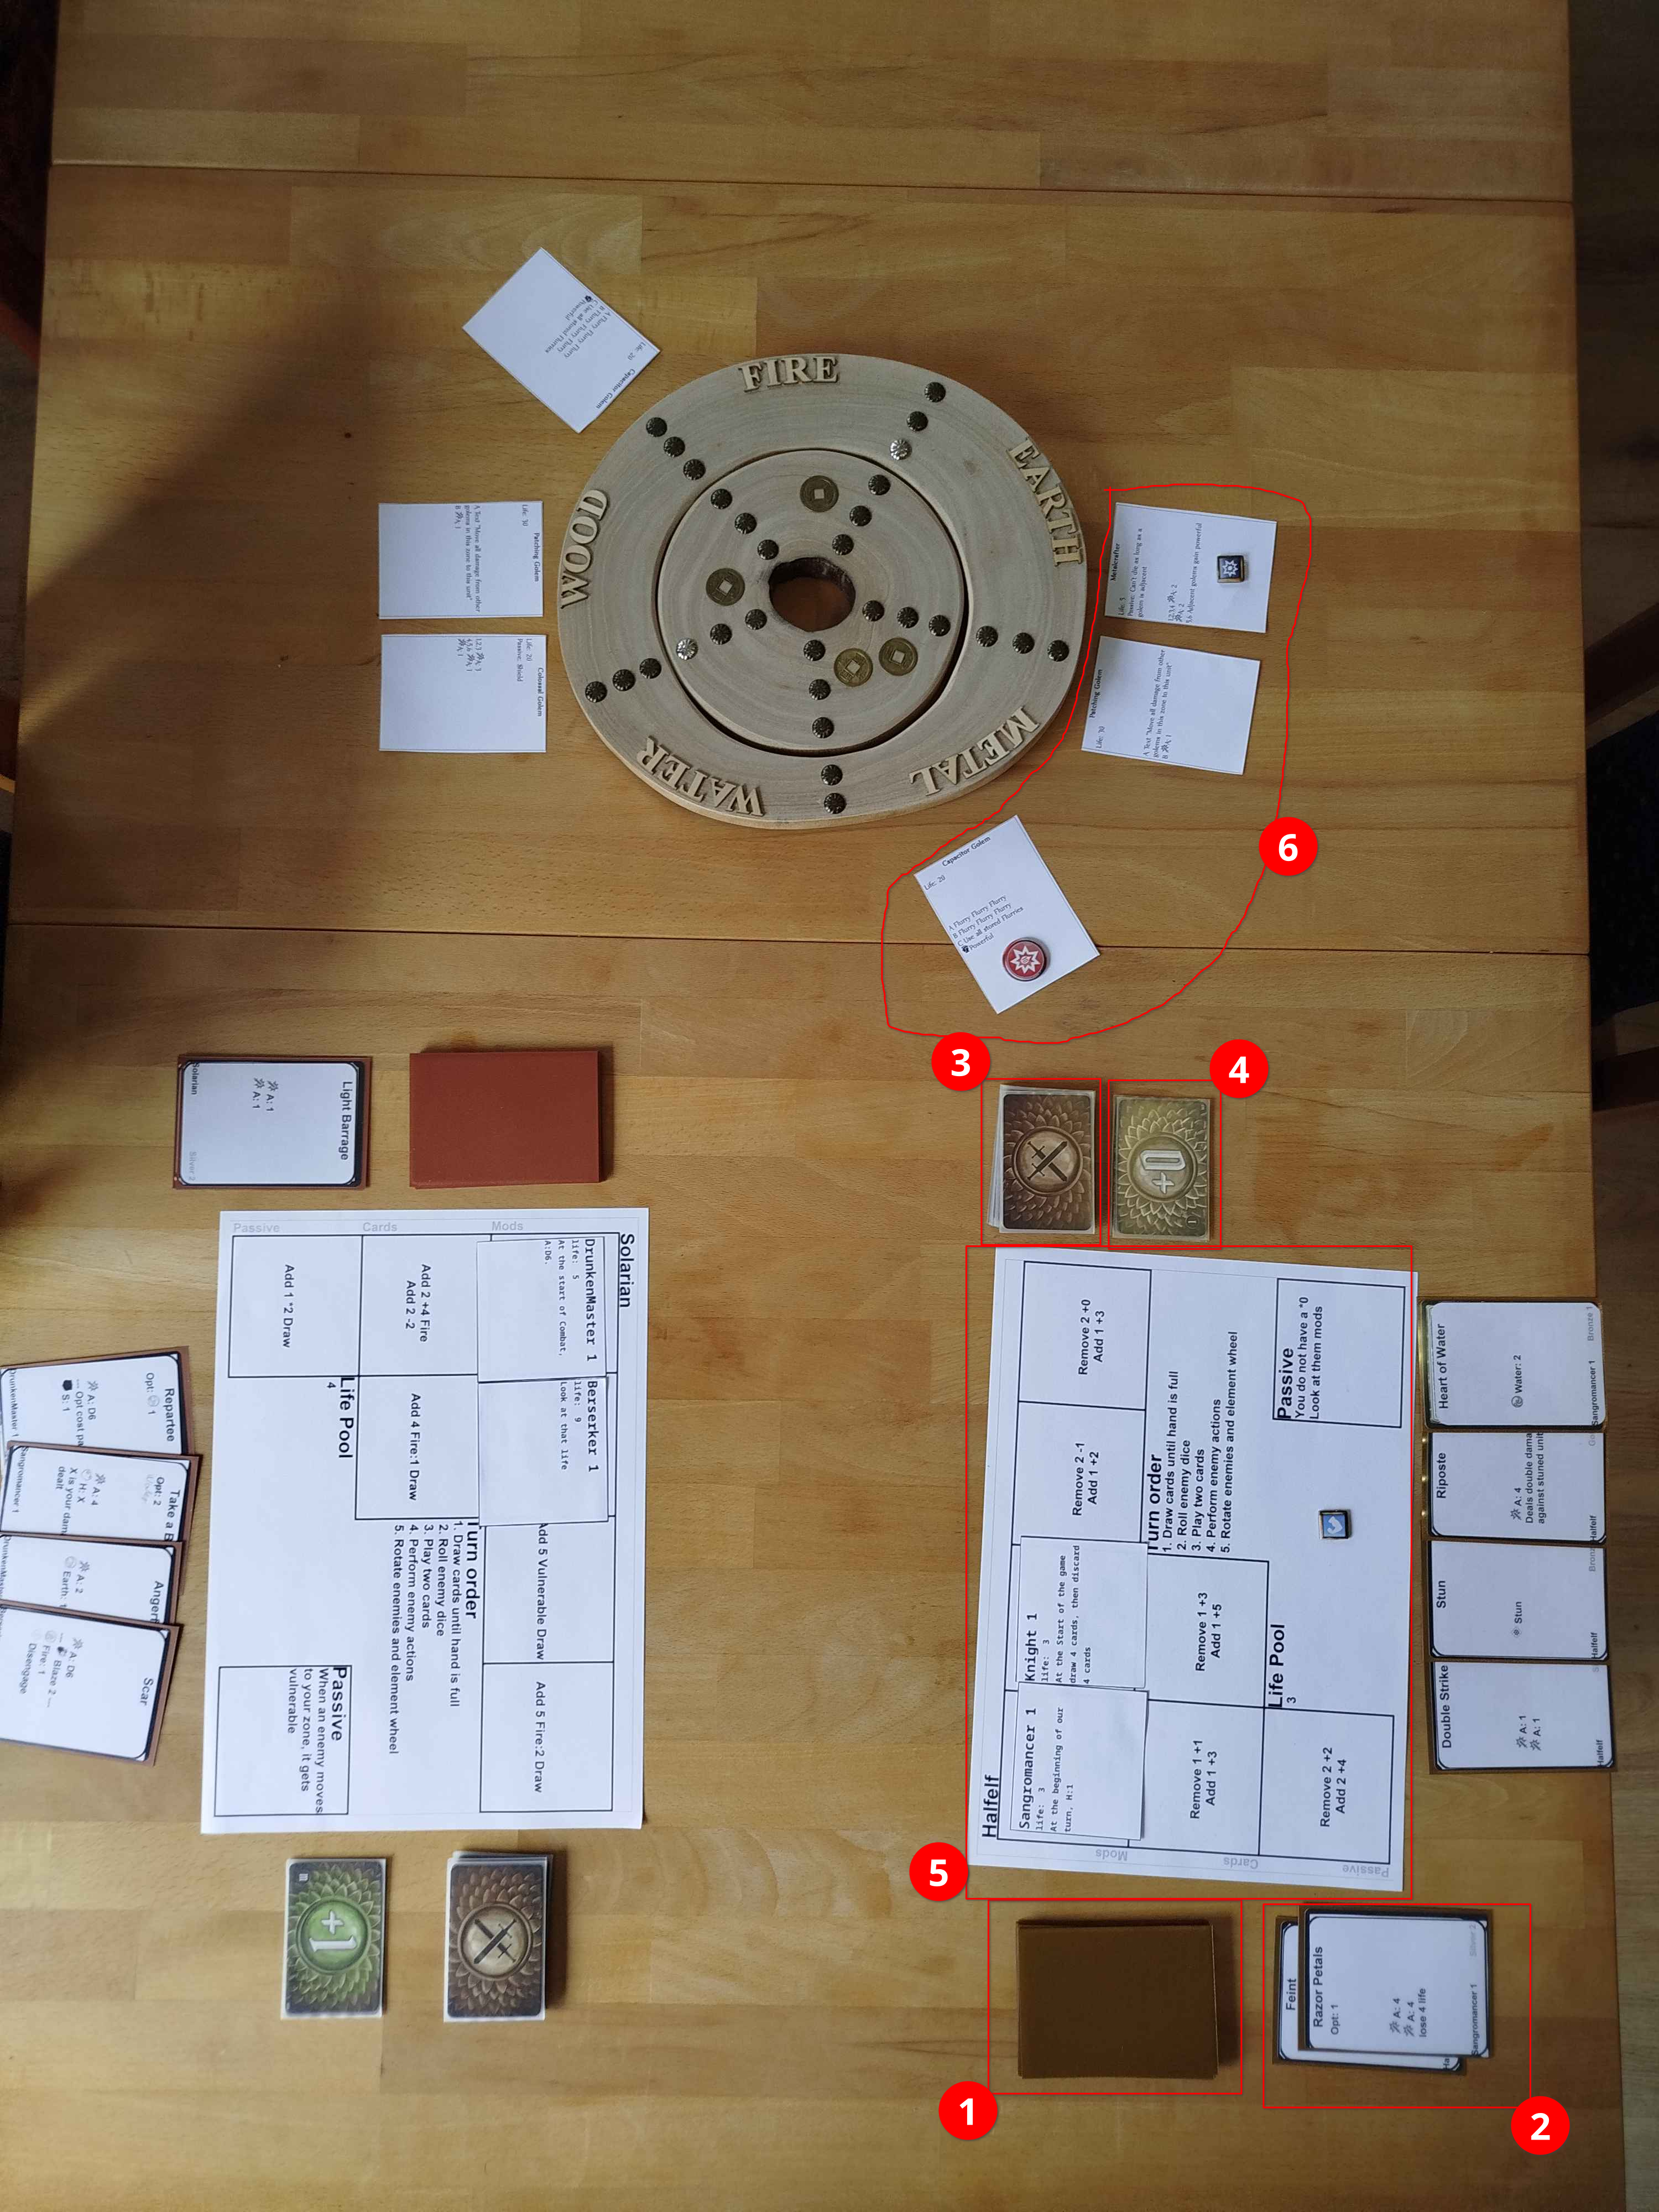
\includegraphics[width=0.9\linewidth, valign=t]{ExplanationPics/PlayAreaAnnotated.png}
	\end{minipage}
	\begin{minipage}[t][10cm][t]{0.5\textwidth}
		\begin{enumerate}	
			\item \textbf{Action draw pile} - Shuffle your Action Deck before combat begins to create your draw pile
			\item \textbf{Action discard pile} - After you play a card, it is placed face up in this pile
			\item \textbf{Dice Pool} - All your current Ancestry Dice are being placed here
			\item \textbf{Ancestry Tableau} - The tableau helps you track your decisions as you level up, your health pool, and contains some reminder text for the turn order
			\item \textbf{Enemy Zone} - Enemies go here, with the configuration described in the storybook
			\item \textbf{The Wheel of Elements} - Many cards use a shared resource called elements. This resource is tracked here.
			\item \textbf{The Storybook} - This book contains the story and encounter setup 
			\item \textbf{The Event Deck} - Between encounters, events will be drawn from this deck to mix up the way the following encounters unfold
		\end{enumerate}
		
		\fbox{\parbox[4cm]{\textwidth}{Picture:  Silverkin, sorting stacks of archaic thick playing cards}}
		
	\end{minipage}	
	
	%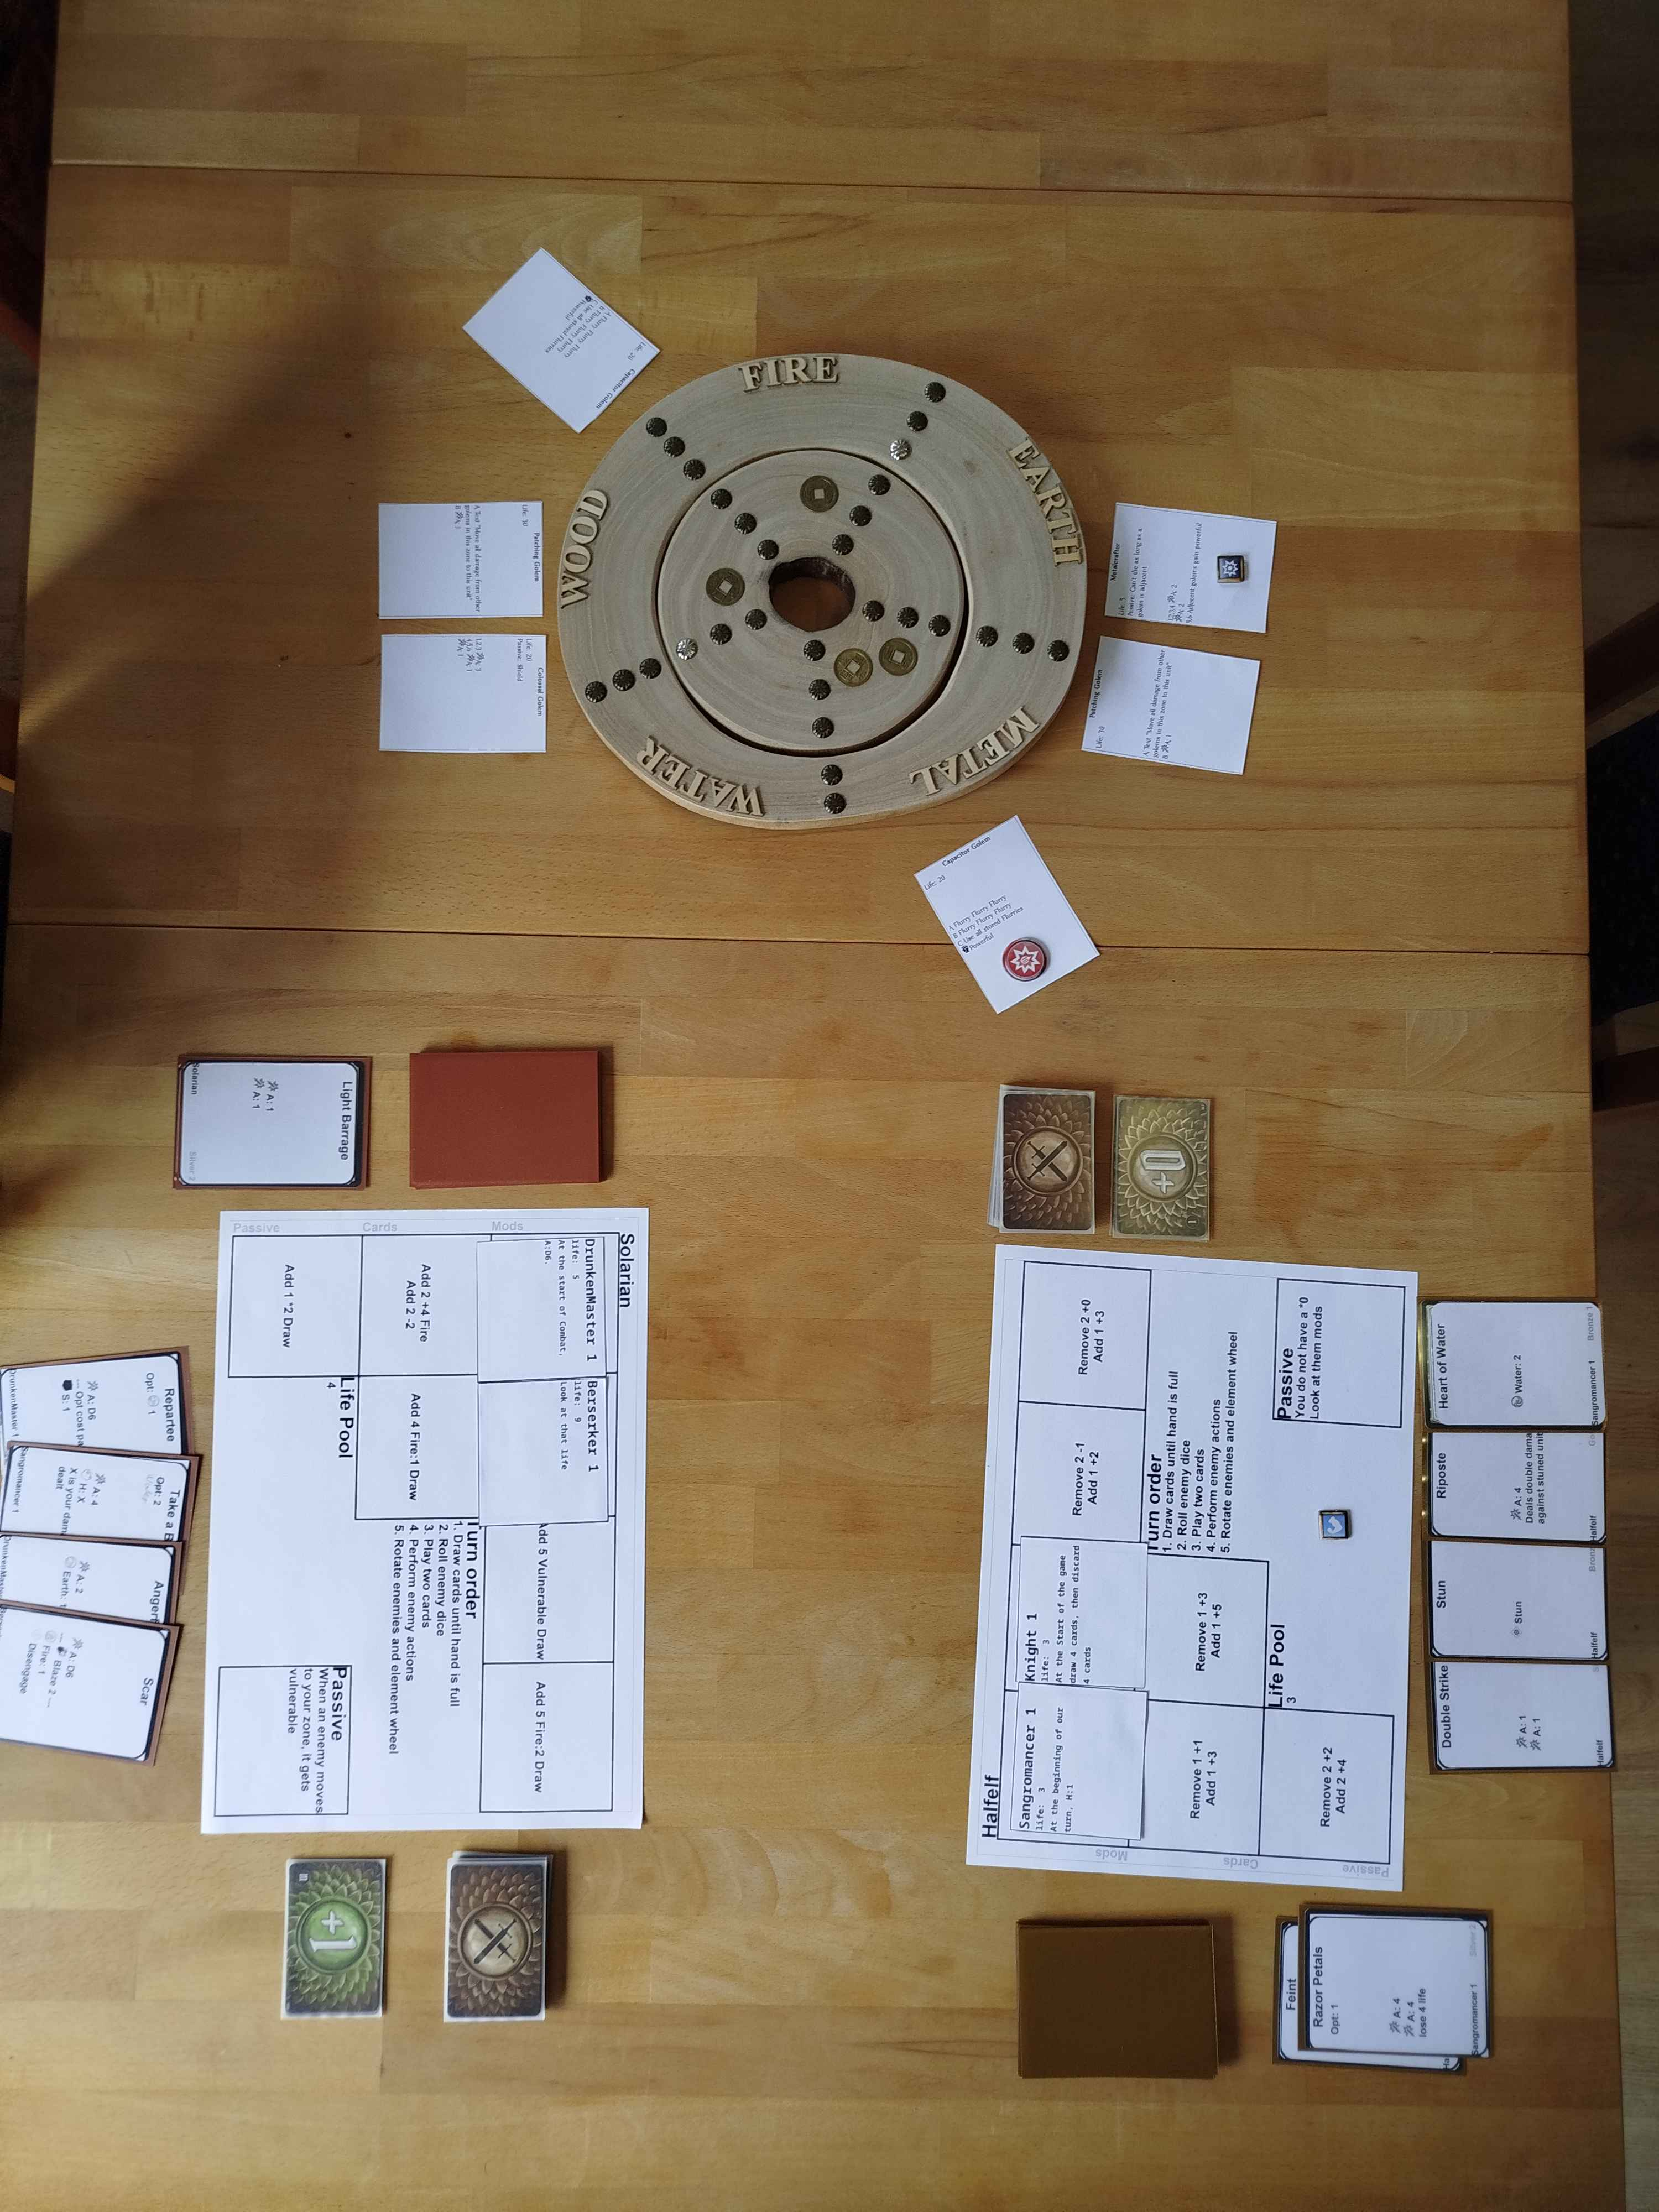
\includegraphics[width=0.8\textwidth]{ExplanationPics/TwoBoards.jpg}
\end{figure}


\section{Setup}

\begin{minipage}[t][10cm][t]{0.5\textwidth}
	To construct their first action and modifier deck, each \textbf{player} follows these steps:
	\begin{enumerate}	
		\item \textbf{Species} - Pick an Ancestry
		\item \textbf{Class 1} - Pick your first rank 1 class
		\item \textbf{Class 2} - Pick a second rank 1 class
		\item \textbf{Action Deck} - Shuffle all action cards from your species and two classes together. This forms your Action Deck
		\item \textbf{Ancestry Tableau} - Take your chosen Ancestry Tableau
		\item \textbf{Ancestry Dice} - Take the ancestry dice indicated by the top left rectangular slot on your Ancestry tableau
		\item \textbf{Class Tiles} - Place the two Class Tiles you chose into the top left rectangular slot on your Ancestry Tableau
		\item \textbf{Ancestry Dice} - Calculate your starting life by adding all totals from your ancestry and the two classes. Place a life marker on the corresponding position.
	\end{enumerate}
	
	
	\vspace{0.3cm}
	The \textbf{shared} play area is constructed as follows:
	\begin{enumerate}
		\item \textbf{Wheel} - Put the Wheel of Elements in the middle
		\item \textbf{Storybook} - Select a new story from the Storybook (We recommend Story Nr.1 if it is everyone's first time playing)
		\item \textbf{Story} - Read out the first passage of the story
		\item \textbf{Encounter} - Set up the enemies corresponding to the first encounter description
	\end{enumerate}
\end{minipage}	
\subsection*{Setup for encounters 2 and 3}
After you beat each encounter, you level up, as described on page \pageref{Section_CharacterBuilding}.
Do some deckbuilding, and you proceed to the next encounter.
After the first encounter, read out passage 2 from the storybook and set up the second encounter.
When beating encounter 2, repeat with passage 3 and encounter 3, and when you beat encounter 3,  read the last passage from the story. When you reach this point, you win.
